\documentclass[11pt]{article}

\usepackage[T1]{fontenc}
\usepackage[polish]{babel}
\usepackage[utf8]{inputenc}
\usepackage{lmodern}
\usepackage{amsfonts}
\usepackage{enumerate}
\usepackage{graphicx}
\usepackage{float}
\usepackage[margin=1in]{geometry}

\selectlanguage{polish}
\graphicspath{{../images/}}

\begin{document}
\title{Sprawozdanie 123}
\author{Jacek Gosztyła, Antoni Mleczko}
\maketitle
\section{Cel ćwiczenia} 
Poznanie własności warstwowych złącz półprzewodnikowych typu p-n. Wyznaczenie charakterystyki stało prądowej różnego rodzaju diod. 
\section{Wstęp teoretyczny}
Ze względu na różnice konduktywności (przewodzenie elektrycznego) możemy podzielić ciała na: 
\begin{itemize}
\item przewodniki - dobrze przewodzą prąd elektryczny
\item półprzewodniki - konduktywność może być zmieniana poprzez domieszkowanie, ogrzewanie i inne czynniki
\item izolatory - nie przewodzą prądu. 
\end{itemize}

Nośniki ładunku w przewodnikach i półprzewodnikach możemy podzielić na elektrony i dziury. \\
Nośniki możemy stworzyć dodając odpowiednie substancje. Dodając akceptory które popierają elektrony, zwiększamy ilość dziur które przy dużej ilości akceptorów stają się nośnikiem większościowym. \\
Żeby zwiększyć liczbą nośników elektronów, musimy użyć  domieszki donorowej - ona dodaje elektrony. \\
W półprzewodniku samoistnym (bez domieszek) koncentracje elektronów n i dziur p są równe. \\
Charakterystyka prądowo napięciowa złącza p - n jest nie liniowa. Dobrze przewodzi w kierunku przewodzenia, natomiast prawie w ogóle nie przewodzi w  kierunku zaporowym.  \\ 
Gdy na końce złącza p-n przyłożymy napięcie w kierunku przewodzenia, dziury będą mogły się swobodnie przemieszczać. W przeciwnym wypadku będą przemieszczać się tylko nośniki mniejszościowe, a więc prąd nie będzie płynął. 



Kierunek przewodzenia / zaporowy.
Polaryzacja przewodzenia - 
Charakterystyka prądowo-napięciowa. 
Współczynnik idealności.
Przesunięcie charakterystyk diody krzemowej względem germanowej. 
Przerwa energetyczna. 
Określenie materiału z jakiego wykonana jest dioda. 
Dioda germanowa, dioda Zenera, dioda świecąca. 
Polaryzacja zaporowa. 
Napięcie stabilizowane.
Współczynnik stabilizacji. 

\section{Realizacja doświadczenia}
\subsection{Pomiary}
Pomiary załączamy do sprawozdania.
\subsection{Opracowanie wyników pomiarów}
\subsubsection{Kierunek przewodzenia}
\begin{figure}[H]
    \centering
    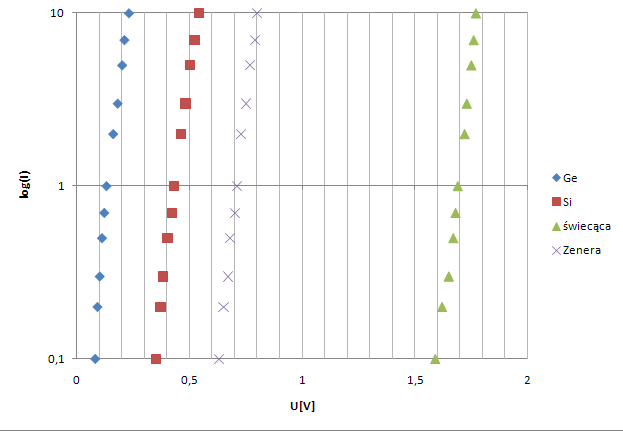
\includegraphics[height=0.27\paperheight]{graph1}
    \caption{ Wspólny  wykres  charakterystyk  prądowo-
napięciowych dla 4 typów diod,  $log(I) = f(U)$  dla  wszystkich  zmierzonych  diod. Oznaczenie jak na rysunku. }
    \label{fig:graph3}
\end{figure}

\begin{figure}[H]
    \centering
    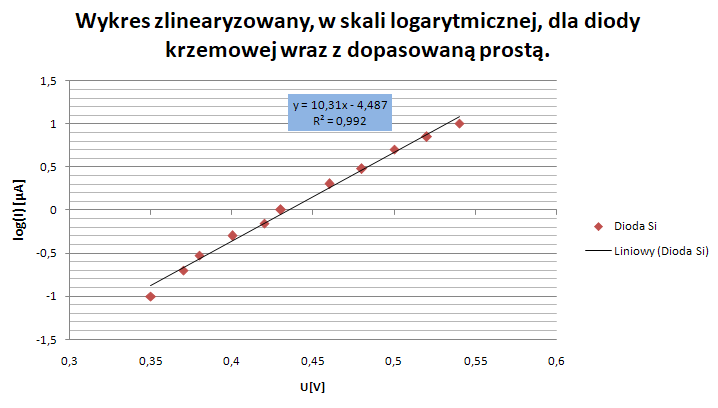
\includegraphics[height=0.27\paperheight]{graph2}
    \caption{ Wykres  zlinearyzowany $ log(I) = f(U)$ dla diody krzemowej wraz z dopasowaną prostą. }
    \label{fig:graph3}
\end{figure}
\subsubsection{Kierunek zaporowy}
\section{Wnioski}

\end{document}

